% Phase-III Report -- EcoGraph: Graph Based Algorithmic Waste Management
% Built on the department-supplied Phase-3.tex progress template.
% Compile with pdfLaTeX. geulogo.png and the member photos (tejas.jpeg, apoorv.jpeg, yash.jpeg) sit in this folder.

\documentclass[12pt,a4paper]{article}

% ============================================================
% PACKAGES
% ============================================================
\usepackage[
    a4paper,
    top=1.55cm,
    bottom=1.35cm,
    left=1.75cm,
    right=1.75cm
]{geometry}

\usepackage[T1]{fontenc}
\usepackage{newtxtext}
\usepackage{graphicx}
\usepackage{xcolor}
\usepackage{array}
\usepackage{tabularx}
\usepackage{fancyhdr}
\usepackage{tikz}
\usepackage{eso-pic}
\usepackage{ragged2e}
\usepackage{enumitem}
\usepackage{amsmath}
\usepackage[hidelinks]{hyperref}
\usetikzlibrary{positioning,arrows.meta,decorations.pathreplacing,calc}

\definecolor{DiagFill}{RGB}{238,244,251}
\definecolor{DiagGrey}{RGB}{90,90,90}

% plain-language formula block: \formula{line \\ line}
\newcommand{\formula}[1]{%
    \begin{center}
    \colorbox{DiagFill}{\parbox{0.92\linewidth}{\vspace{4pt}\centering\fontsize{10}{14}\selectfont #1\vspace{4pt}}}
    \end{center}
}

% boxed figure that continues the Approach section: \diagbox{title}{body}
\newcommand{\diagbox}[2]{%
    \par\noindent
    \fbox{\begin{minipage}{\dimexpr\textwidth-2\fboxsep-2\fboxrule\relax}
        \vspace{4pt}
        {\color{GEUBlue}\bfseries\fontsize{11.5}{14}\selectfont #1}
        \vspace{4pt}

        \fontsize{10}{12.5}\selectfont
        #2
        \vspace{4pt}
    \end{minipage}}\par
}

% ============================================================
% COLORS
% ============================================================
\definecolor{GEUBlue}{RGB}{43,91,145}
\definecolor{GEUBannerBlue}{RGB}{0,102,148}
\definecolor{GEUYellow}{RGB}{255,201,38}
\definecolor{InstructionGrey}{RGB}{125,125,125}

% ============================================================
% GENERAL SETTINGS
% ============================================================
\setlength{\parindent}{0pt}
\setlength{\parskip}{0pt}
\renewcommand{\arraystretch}{1}
\setlist{leftmargin=5mm,itemsep=1pt,topsep=2pt,parsep=0pt}

% ============================================================
% HEADER / FOOTER
% ============================================================
\pagestyle{fancy}
\fancyhf{}

\fancyhead[L]{%
    \fontsize{10.5}{12}\selectfont
    DSA \& OOPs in C++ (DSCPP) -- Team DSCPP-III-2026-T186
}

\fancyhead[R]{%
    \fontsize{10.5}{12}\selectfont
    PHASE-III PROJECT PROGRESS
}

\fancyfoot[R]{%
    \fontsize{10}{12}\selectfont
    Page \thepage
}

\renewcommand{\headrulewidth}{0pt}
\renewcommand{\footrulewidth}{0pt}

\setlength{\headheight}{20pt}
\setlength{\headsep}{0.65cm}
\setlength{\footskip}{0.65cm}

% ============================================================
% BOTTOM YELLOW LINE
% ============================================================
\AddToShipoutPictureBG{%
\begin{tikzpicture}[remember picture,overlay]
    \fill[GEUYellow]
    (current page.south west)
    rectangle
    ([yshift=0.14cm]current page.south east);
\end{tikzpicture}
}

% ============================================================
% CUSTOM COMMANDS
% ============================================================
\newcommand{\sectiontitle}[1]{%
    {\color{GEUBlue}
    \fontsize{18}{22}\selectfont #1}
}

\newcommand{\instruction}[1]{%
    {\color{InstructionGrey}
    \fontsize{10.5}{13}\selectfont #1}
}

\newcommand{\answerbox}[2]{%
    \begin{tabularx}{\textwidth}{
        |>{\raggedright\arraybackslash}X|}
        \hline
        \parbox[t][#1][t]{\dimexpr\linewidth-12pt\relax}{
            \vspace{5pt}
            \fontsize{11}{13.5}\selectfont
            \setlength{\parskip}{4pt}
            #2
        }\\
        \hline
    \end{tabularx}
}

% one row of the two-column task tables
\newcommand{\taskrow}[2]{%
    \parbox[t]{\linewidth}{\vspace{3pt}\fontsize{10.5}{12.5}\selectfont #1\vspace{4pt}}
    &
    \parbox[t]{\linewidth}{\raggedright\vspace{3pt}\fontsize{10.5}{12.5}\selectfont #2\vspace{4pt}}
    \\
    \hline
}

% natural-height answer box (long answers set their own height)
\renewcommand{\answerbox}[1]{%
    \noindent\fbox{\begin{minipage}{\dimexpr\textwidth-2\fboxsep-2\fboxrule\relax}
        \vspace{3pt}
        \fontsize{11}{13.5}\selectfont
        \setlength{\parskip}{4pt}
        #1
        \vspace{3pt}
    \end{minipage}}\par
}

% one row of the team table: role, name, ID, roll, email, photo
\newcommand{\memberrow}[6]{%
    \begin{minipage}[t]{\linewidth}
    \vspace{1.5mm}
    \textbf{#1}
    \vspace{1.5mm}
    \end{minipage}
    &
    \begin{minipage}[t]{\linewidth}
    \vspace{1.5mm}
    \fontsize{11}{13}\selectfont
    \textit{#2}\\
    \textit{Student ID: #3}\\
    \textit{Roll No. #4}\\
    \textit{#5}

    \vspace{1mm}
    \includegraphics[width=3.0cm,height=2.15cm,keepaspectratio]{#6}
    \vspace{1mm}
    \end{minipage}
    \\
    \hline
}

% one row of the testing table (every row ran and passed)
\newcommand{\testrow}[2]{%
    \parbox[t]{\linewidth}{\raggedright\vspace{3pt}\small #1\vspace{3pt}} & \parbox[t]{\linewidth}{\vspace{3pt}\small Pass} & \parbox[t]{\linewidth}{\raggedright\vspace{3pt}\small #2\vspace{3pt}}\\ \hline
}

% one framed screenshot with a caption: \shot{file}{caption}
\newcommand{\shot}[2]{%
    {\centering\fbox{\includegraphics[width=\dimexpr\textwidth-2\fboxsep-2\fboxrule\relax,height=10.6cm,keepaspectratio]{#1}}\par}
    \vspace{1mm}
    {\fontsize{10}{12}\selectfont #2\par}
}

% ============================================================
% DOCUMENT
% ============================================================
\begin{document}

% ============================================================
% PAGE 1
% ============================================================

\vspace*{0.10cm}


\includegraphics[width=8.0cm]{geulogo.png}

\vspace{0.40cm}

\noindent
\colorbox{GEUBannerBlue}{%
\parbox{\dimexpr\textwidth-2\fboxsep\relax}{
    \vspace{0.17cm}
    {\color{GEUYellow}
    \fontsize{16.5}{20}\selectfont
    \bfseries
    PROJECT AND TEAM INFORMATION}
    \vspace{0.17cm}
}}

\vspace{0.40cm}

% PROJECT TITLE
\sectiontitle{Project Title}

\vspace{0.20cm}

\answerbox{EcoRouting Engine: Hazard-Aware Path Optimization and Fill-Rate-Adaptive Waste Scheduling}

\vspace{0.40cm}

% TEAM INFORMATION
\sectiontitle{Student/Team Information}

\vspace{0.20cm}

\noindent
\begin{tabularx}{\textwidth}{|>{\RaggedRight\arraybackslash}p{0.60\textwidth}|>{\RaggedRight\arraybackslash}X|}
\hline
\begin{minipage}[t]{\linewidth}
\vspace{1.5mm}
\textit{Team Name:}\\[-1mm]
\textit{Team \#}\\[-1mm]
\textit{PBL Mentor:}
\vspace{1.5mm}
\end{minipage}
&
\begin{minipage}[t]{\linewidth}
\vspace{1.5mm}
\textit{EcoGraph}\\[-1mm]
\textit{DSCPP-III-2026-T186}\\[-1mm]
\textit{Mr. Navneet Rajput}
\vspace{1.5mm}
\end{minipage}
\\
\hline
\memberrow{Team member 1 (Team Lead)}{Jain, Tejas}{2510011541}{2028228, Sec A}{aispace101@gmail.com}{tejas.jpeg}
\memberrow{Team member 2}{Negi, Apoorv}{2510011088}{2027640, Sec D}{apoorvnegi17@gmail.com}{apoorv.jpeg}
\memberrow{Team member 3}{Nigam, Yash}{2510010441}{2028289, Sec H}{nigamyash07@gmail.com}{yash.jpeg}
\end{tabularx}

\newpage
% ============================================================
% PAGE 2
% ============================================================

\vspace*{0.15cm}

\noindent
\colorbox{GEUBannerBlue}{%
\parbox{\dimexpr\textwidth-2\fboxsep\relax}{
    \vspace{0.18cm}
    {\color{GEUYellow}
    \fontsize{17}{21}\selectfont
    \bfseries
    PHASE-III PROJECT PROGRESS DESCRIPTION}
    \vspace{0.18cm}
}}

\vspace{0.50cm}

% ABSTRACT
\sectiontitle{Project Abstract}

\vspace{0.12cm}

\answerbox{Anyone who has watched a municipal garbage truck on its route notices the same thing: it drives the same streets every day, in the same order, whether or not there is anything to collect. Routes are fixed by habit rather than the actual shortest path between the depot, the homes on the list, and the disposal sites, wasting fuel, driver time, and public money. Two problems compound this. Hazardous waste -- medical sharps, expired chemicals, batteries -- is often collected the same way as ordinary household waste, even though it should be picked up immediately and kept off residential and commercial streets on its way to disposal; delays or careless routing here are a genuine safety and environmental risk. Second, every disposal site is treated as if it fills at the same rate, so a fixed weekly schedule either visits a disposal site that is nowhere near full or leaves an overflowing one unattended. We wanted a system that treats the city as the graph it actually is, and routes, restricts, and schedules collection accordingly.

Our project is a working C++ backend that models the city as a weighted, zone-tagged graph and answers three questions on demand: the shortest route to collect from a given set of homes, which locations are actually due today based on fill-rate, and how to route hazardous waste safely away from residential streets -- all exposed through a REST API and shown live on a PixiJS frontend that animates the computed route. The system is hosted at \href{https://ecograph-xl8q.onrender.com}{\texttt{ecograph-xl8q.onrender.com}}.}

\newpage

% UPDATED APPROACH
\vspace*{0.20cm}

\sectiontitle{Updated Project Approach and Architecture}

\vspace{0.12cm}

\answerbox{\textbf{Design.} One C++17 process serves the REST API and the front end on one port. \texttt{controllers.cpp} handles HTTP and JSON behind a mutex; domain classes (\texttt{Graph}, Dijkstra, \texttt{Scheduler}, classifier, route builders, \texttt{Simulation}) work on an in-memory adjacency-list city loaded from \texttt{city.json}.

\textbf{Routing.} \texttt{RouteStrategy} is an abstract base class; its Priority subclass sets the stop order (priority mode: the fullest home comes first).

\textbf{Protocol.} REST over HTTP with JSON, 15 endpoints, one error format.

\textbf{Front end.} Plain JavaScript with no build step, plus a day-by-day simulation and a limited fleet.

\textbf{Libraries.} cpp-httplib, nlohmann/json, PixiJS.

\textbf{Deployment.} A multi-stage Docker image compiles the server, then copies only the binary, \texttt{city.json} and the front end into a slim runtime image. It runs as one long-lived container on Render, with the front end on the same origin as the API.

\vspace{1mm}
{\color{GEUBlue}\bfseries\fontsize{12}{14}\selectfont System overview} \quad {\small(diagrams (a)--(g) on the next pages)}

\textbf{1.} The clock moves forward one day.

\textbf{2.} A home is due once the days since its last collection reach capacity / fill rate (1--14 days); the fullest home comes first (c).

\textbf{3.} Due disposal sites are emptied, hazardous homes go to the hazard trucks (f), and normal homes are ordered and packed onto trucks before routing (e).

\textbf{4.} Each truck chains shortest paths in its list order:
\formula{\raggedright\ttfamily\small
current = DEPOT;\ \ visited = \{ \}\\
for each home in order:\\
\hspace*{4mm}skip it if in visited\\
\hspace*{4mm}path = Dijkstra(current $\to$ home);\ \ if none, mark unreachable\\
\hspace*{4mm}empty later stops on the path, add them to visited\hfill\textrm{\small(en-route pickup, (d))}\\
\hspace*{4mm}empty home, add to visited;\ \ current = home\\
then visit the nearest disposal site for each waste type collected}

\textbf{5.} Served homes get ``last collected = today''; unreachable ones are reported as failed, and carried-over homes rank higher tomorrow.}

\newpage

% ------------------------------------------------------------
% APPROACH: DIAGRAMS
% ------------------------------------------------------------

\diagbox{(a) System Pipeline}{%
\begin{center}
\begin{tikzpicture}[
node distance=8mm,
box/.style={rectangle,rounded corners,draw=GEUBlue,fill=DiagFill,thick,minimum width=2.4cm,minimum height=12mm,align=center,font=\scriptsize\sffamily},
arrow/.style={-{Latex[length=2mm]},thick,draw=GEUBlue}
]
\node[box] (a) {Browser UI\\JS + PixiJS};
\node[box,right=of a] (b) {HTTP layer\\cpp-httplib};
\node[box,right=of b] (c) {Controllers\\JSON + mutex};
\node[box,right=of c] (d) {Domain classes\\Graph, Dijkstra,\\Router, Scheduler,\\Simulation};
\node[box,right=of d] (e) {In-memory\\city state};
\node[box,below=6mm of e] (f) {\texttt{city.json}};
\draw[arrow] (a)--node[above,font=\tiny]{REST}(b);
\draw[arrow] (b)--(c); \draw[arrow] (c)--(d); \draw[arrow] (d)--(e);
\draw[arrow] (f)--node[right,font=\tiny]{load once}(e);
\end{tikzpicture}
\end{center}}

\vspace{0.35cm}

\diagbox{(b) Graph Storage and Dijkstra}{%
\begin{center}
\begin{tikzpicture}[
node distance=13mm,
nd/.style={draw=GEUBlue,fill=DiagFill,thick,rounded corners,minimum width=1.3cm,minimum height=7mm,font=\scriptsize,align=center},
lbl/.style={font=\tiny,draw=none,fill=none}
]
\node[nd] (depot) {DEPOT};
\node[nd,right=of depot] (j1) {J1};
\node[nd,right=of j1] (h1) {H1};
\node[nd,right=of h1] (b1) {B1};
\draw[thick,GEUBlue] (depot)--(j1) node[midway,above,lbl]{4.2 km};
\draw[thick,GEUBlue] (j1)--(h1) node[midway,above,lbl]{3.1 km};
\draw[thick,GEUBlue] (h1)--(b1) node[midway,above,lbl]{6.0 km};
\end{tikzpicture}

\vspace{3mm}
\begin{tikzpicture}[
node distance=7mm,
box/.style={rectangle,rounded corners,draw=GEUBlue,fill=DiagFill,thick,minimum width=2.4cm,minimum height=9mm,align=center,font=\scriptsize\sffamily},
arrow/.style={-{Latex[length=2mm]},thick,draw=GEUBlue}
]
\node[box] (a) {Init \texttt{dist[]},\\push source};
\node[box,right=of a] (b) {Pop min-dist\\node $u$};
\node[box,right=of b] (c) {Relax edges\\of $u$};
\node[box,right=of c] (d) {Rebuild path\\from \texttt{prev[]}};
\draw[arrow] (a)--(b); \draw[arrow] (b)--(c); \draw[arrow] (c)--(d);
\draw[arrow] (c.north) to[out=90,in=90] node[midway,above,font=\tiny]{until heap empty} (b.north);
\end{tikzpicture}
\end{center}}

\vspace{0.35cm}

\diagbox{(c) Fill-Rate Scheduling}{%
\begin{center}
\begin{tikzpicture}[font=\scriptsize]
\draw[thick,GEUBlue,-{Latex[length=2mm]}] (0,0) -- (14,0) node[right]{days};
\draw[thick,GEUBlue] (0,0.15) -- (0,-0.15) node[below,yshift=-1mm]{last collected};
\draw[thick,GEUBlue] (7,0.15) -- (7,-0.15) node[below,yshift=-1mm]{due day = last collected + interval};
\draw[thick,red] (11,0.15) -- (11,-0.15) node[below,yshift=-1mm]{now};
\draw[decorate,decoration={brace,amplitude=4pt},thick,red] (7,0.4) -- (11,0.4) node[midway,above,yshift=2mm]{overdue by $\to$ rank in max-heap};
\node[above] at (3.5,0) {interval};
\end{tikzpicture}
\end{center}}

\vspace{0.35cm}

\diagbox{(d) En-Route Pickup}{%
\begin{center}
\begin{tikzpicture}[
nd/.style={circle,draw=GEUBlue,fill=DiagFill,thick,minimum size=8mm,font=\scriptsize\bfseries},
lbl/.style={font=\tiny,draw=none,fill=none}
]
% literal order
\node[font=\scriptsize\bfseries,anchor=west] at (-0.4,2.1) {Literal order A $\to$ C $\to$ B: 6 km};
\node[nd] (a1) at (0,0) {A};
\node[nd] (b1) at (2.6,0) {B};
\node[nd] (c1) at (5.2,0) {C};
\draw[thick,GEUBlue!40] (a1)--(b1) node[midway,below,lbl]{2 km};
\draw[thick,GEUBlue!40] (b1)--(c1) node[midway,below,lbl]{2 km};
\draw[-{Latex[length=2mm]},thick,GEUBlue] (a1) to[out=40,in=140] node[midway,above,lbl]{passes B without stopping} (c1);
\draw[-{Latex[length=2mm]},thick,red,dashed] (c1) to[out=-140,in=-40] node[midway,below,lbl]{back for B (+2 km)} (b1);
% en-route
\node[font=\scriptsize\bfseries,anchor=west] at (8.0,2.1) {EcoGraph: A $\to$ B $\to$ C: 4 km};
\node[nd] (a2) at (8.4,0) {A};
\node[nd,fill=green!20,draw=green!45!black] (b2) at (11.0,0) {B};
\node[nd] (c2) at (13.6,0) {C};
\draw[-{Latex[length=2mm]},thick,green!45!black] (a2)--(b2) node[midway,below,lbl]{2 km};
\draw[-{Latex[length=2mm]},thick,green!45!black] (b2)--(c2) node[midway,below,lbl]{2 km};
\node[lbl,below=1mm of b2] {collected en route};
\end{tikzpicture}
\end{center}}

\vspace{0.35cm}

\diagbox{(e) Truck Fleet and Capacity}{%
\begin{center}
\begin{tikzpicture}[
node distance=5mm and 6mm,
box/.style={rectangle,rounded corners,draw=GEUBlue,fill=DiagFill,thick,minimum width=2.7cm,minimum height=10mm,align=center,font=\scriptsize\sffamily},
hz/.style={box,draw=red!70!black,fill=red!6},
bad/.style={box,draw=DiagGrey,fill=white,dashed},
arrow/.style={-{Latex[length=2mm]},thick,draw=GEUBlue}
]
\node[box,yshift=-7mm] (due) {Today's due list\\(max-heap)};
\node[box,right=of due,yshift=20mm] (bins) {Due disposal\\sites};
\node[box,right=of due,yshift=7mm] (norm) {Normal homes};
\node[hz,right=of due,yshift=-27mm] (haz) {Hazardous homes};
\node[box,right=of bins] (emp) {Emptied in place};
\node[box,right=of norm] (ord) {\texttt{order()}\\Priority};
\node[box,right=of ord] (ff) {First-fit into\\trucks N1, N2, \ldots\\(up to 1000 kg)};
\node[box,right=of ff,minimum width=2.3cm] (rt) {\texttt{buildRoute()}\\per truck};
\node[hz,right=of haz] (fifo) {Earliest due\\first};
\node[hz,right=of fifo] (ht) {HT1, HT2\\one trip each};
\node[hz,right=of ht,minimum width=2.3cm] (dh) {\texttt{dispatch}\\\texttt{Hazard()}};
\node[bad,below=5mm of ff] (co) {\texttt{carriedOver}\\(next day)};
\draw[arrow] (due.east)--++(3mm,0)|-(bins.west);
\draw[arrow] (due.east)--++(3mm,0)|-(norm.west);
\draw[arrow] (due.east)--++(3mm,0)|-(haz.west);
\draw[arrow] (bins)--(emp); \draw[arrow] (norm)--(ord); \draw[arrow] (ord)--(ff); \draw[arrow] (ff)--(rt);
\draw[arrow,red!70!black] (haz)--(fifo); \draw[arrow,red!70!black] (fifo)--(ht); \draw[arrow,red!70!black] (ht)--(dh);
\draw[arrow,dashed,DiagGrey] (ff)--node[right,font=\tiny]{no room}(co);
\draw[arrow,dashed,DiagGrey] (ht.north)--node[right,font=\tiny]{trucks used up}(co.south);
\end{tikzpicture}
\end{center}}

\vspace{0.35cm}

\diagbox{(f) Automatic Hazard Dispatch and Risk-Weighted Dijkstra}{%
\begin{center}
\begin{tikzpicture}[
node distance=11mm,
box/.style={rectangle,rounded corners,draw=GEUBlue,fill=DiagFill,thick,minimum width=2.3cm,minimum height=10mm,align=center,font=\scriptsize\sffamily},
hz/.style={box,draw=red!70!black,fill=red!6},
arrow/.style={-{Latex[length=2mm]},thick,draw=GEUBlue}
]
\node[box] (w) {Waste\\description};
\node[box,right=of w] (cl) {Classifier\\keyword match};
\node[hz,right=of cl] (d1) {Depot $\to$ home\\avoids res./comm. roads};
\node[hz,right=of d1] (d2) {Home $\to$ nearest\\disposal site};
\node[hz,right=of d2] (tr) {Hazard truck\\HT1 / HT2};
\node[box,below=5mm of cl] (nq) {Normal queue};
\draw[arrow] (w)--(cl);
\draw[arrow,red!70!black] (cl)--node[above,font=\tiny]{hazardous}(d1);
\draw[arrow,red!70!black] (d1)--(d2); \draw[arrow,red!70!black] (d2)--(tr);
\draw[arrow] (cl)--node[right,font=\tiny]{not hazardous}(nq);
\end{tikzpicture}

\vspace{3mm}
\begin{tikzpicture}[
nd/.style={draw=GEUBlue,fill=DiagFill,thick,rounded corners,minimum width=1.9cm,minimum height=7mm,font=\scriptsize,align=center},
lbl/.style={font=\tiny,draw=none,fill=none}
]
\node[nd] (j1) at (0,0) {J1 (start)};
\node[nd] (r1) at (4,1.0) {R1 (residential)};
\node[nd] (in1) at (4,-1.0) {IN1 (industrial)};
\node[nd] (bin) at (8,0) {Medical disposal site};
\draw[thick,red,dashed] (j1)--(r1) node[midway,above,sloped,lbl]{2 km $\times$ 15 -- penalised};
\draw[thick,red,dashed] (r1)--(bin) node[midway,above,sloped,lbl]{2 km};
\draw[thick,green!45!black] (j1)--(in1) node[midway,below,sloped,lbl]{5 km -- preferred};
\draw[thick,green!45!black] (in1)--(bin) node[midway,below,sloped,lbl]{3 km};
\end{tikzpicture}
\end{center}}

\vspace{0.35cm}

\diagbox{(g) Simulation Architecture}{%
\begin{center}
\begin{tikzpicture}[
node distance=6mm and 7mm,
box/.style={rectangle,rounded corners,draw=GEUBlue,fill=DiagFill,thick,minimum width=2.6cm,minimum height=10mm,align=center,font=\scriptsize\sffamily},
st/.style={rectangle,draw=GEUBlue,fill=white,thick,minimum width=2.6cm,minimum height=8mm,align=center,font=\scriptsize\sffamily},
arrow/.style={-{Latex[length=2mm]},thick,draw=GEUBlue}
]
% request path
\node[box] (ui) {Simulation panel\\Step / Play / Reset};
\node[box,right=of ui] (ctl) {\texttt{/simulate/advance}\\validate, lock mutex};
\node[box,right=of ctl,minimum width=3.0cm] (sim) {\texttt{Simulation}\\\texttt{advanceDay()} $\times$ days};
\node[box,right=of sim] (rep) {\texttt{DayReport}[]\\as JSON};
\draw[arrow] (ui)--node[above,font=\tiny]{POST}(ctl);
\draw[arrow] (ctl)--(sim);
\draw[arrow] (sim)--(rep);
\draw[arrow] (rep.north) to[bend right=14] node[above,font=\tiny]{animate trucks, refresh map, schedule and database views} (ui.north);
% collaborators
\node[st,below=8mm of ctl,xshift=-1.6cm] (sch) {\texttt{Scheduler}\\due, fill, \%full};
\node[st,right=4mm of sch] (rs) {\texttt{RouteStrategy}\\Priority};
\node[st,right=4mm of rs] (hz) {\texttt{dispatchHazard()}\\constrained Dijkstra};
\node[st,right=4mm of hz] (lg) {Log (last 2000)\\+ \texttt{markCollected()}};
\foreach \n in {sch,rs,hz,lg} \draw[arrow] (sim.south)--(\n.north);
\node[st,below=6mm of rs,xshift=2.0cm,minimum width=4.5cm] (st8) {Shared state: \texttt{Graph} + clock + day};
\foreach \n in {sch,rs,hz,lg} \draw[thick,GEUBlue!50] (\n.south)--(st8.north);
\end{tikzpicture}
\end{center}}
\newpage

% ============================================================
% TASKS COMPLETED
% ============================================================

\vspace*{0.20cm}

\sectiontitle{Tasks Completed}

\vspace{0.20cm}

\begin{tabularx}{\textwidth}{
|>{\raggedright\arraybackslash}X
|>{\raggedright\arraybackslash}p{0.27\textwidth}|
}
\hline
\textbf{Task Completed} &
\textbf{Team Member}\\
\hline
\taskrow{Weighted, zone-tagged city graph as an adjacency list, with a JSON loader for the Dehradun map (70 nodes, 107 roads)}{Tejas Jain (Lead)}
\taskrow{HTTP server on cpp-httplib serving the front end and 15 REST endpoints, with one error format and a mutex on shared state}{Tejas Jain}
\taskrow{Plain and zone-constrained Dijkstra with path rebuilding}{Tejas Jain}
\taskrow{Priority route builder (fullest home first) with en-route pickup and unloading at the nearest disposal site}{Tejas Jain}
\taskrow{Keyword waste classifier and automatic hazard dispatch to the nearest medical or chemical disposal site, keeping off residential and commercial roads wherever another road exists}{Tejas Jain}
\taskrow{Fill-rate scheduler with a max-heap of due locations}{Tejas Jain}
\taskrow{Day-by-day simulation with limited fleet, truck capacity, carry-over and a collection log}{Tejas Jain, Apoorv Negi, Yash Nigam}
\taskrow{Unit test suites for the backend, plus a check of the city data}{Yash Nigam, Apoorv Negi, Tejas Jain}
\taskrow{README with build steps, folder layout and API reference}{Apoorv Negi, Yash Nigam}
\taskrow{PixiJS map view with truck route animation, hazard-route styling and a shape legend}{Yash Nigam, Tejas Jain, Apoorv Negi}
\taskrow{Schedule, simulation and database views and the light/dark theme}{Tejas Jain, Yash Nigam}
\taskrow{Multi-stage Dockerfile and \texttt{.dockerignore}}{Yash Nigam, Tejas Jain}
\taskrow{Deployment on Render as one long-lived container, health check on \texttt{/health}, automatic redeploy from \texttt{main}}{Tejas Jain}
\taskrow{\texttt{PORT}, \texttt{CITY\_FILE} and \texttt{FRONTEND\_DIR} set in the image; front end on the API's origin with \texttt{ECO\_API\_BASE} empty}{Tejas Jain, Yash Nigam}
\taskrow{One-line \texttt{docker run} instructions in the README}{Yash Nigam}
\taskrow{Live demo link in the README}{Tejas Jain}
\taskrow{Front-end improvements}{Tejas Jain}
\taskrow{Code cleanup}{Tejas Jain, Apoorv Negi}
\taskrow{Phase-I and Phase-II reports and presentations}{Apoorv Negi, Yash Nigam}
\end{tabularx}

\newpage

% ============================================================
% CHALLENGES
% ============================================================

\vspace*{0.20cm}

\sectiontitle{Challenges/Roadblocks}

\vspace{0.18cm}

\answerbox{\textbf{Road classes beyond residential and commercial.} If roads were tagged only as residential or commercial, the hazard truck would have no safe road to prefer. Real cities also have main roads between localities and industrial belts where disposal sites sit, so we added \emph{arterial} and \emph{industrial} road classes. The hazard truck's route weights residential roads 15$\times$ and commercial roads 10$\times$, so it crosses the city on these classes and enters a neighbourhood or a market only for the stretch it cannot avoid.

\textbf{Trucks driving past houses on their own list.} At first the router followed the scheduler's order literally: given A, C, B with B on the road from A to C, the truck drove past B, reached C, then turned back for B. We added en-route pickup: each leg's path is checked for later stops, which are emptied on the way and skipped when the list reaches them.

\textbf{Scheduling that never showed its effect.} With unlimited trucks, every due home was served every day, so nothing ever overflowed, and the priority order only changed the stop order, never who got served. We added a limited fleet with 1000 kg per truck and carry-over to the next day. Since an overflowing home heavier than a whole truck would never fit, an empty truck always accepts its first home.

\textbf{Shared state across requests.} cpp-httplib handles requests on several threads, and routing, collection and the simulation all change the same graph, so all shared state sits behind one mutex.

\textbf{Compiler on Windows.} The old MinGW g++ could not build cpp-httplib, which needs proper thread support, so we moved to GCC 13.}

\vspace{0.55cm}

% ============================================================
% OUTCOME
% ============================================================

\sectiontitle{Project Outcome/Deliverables}

\vspace{0.18cm}

\answerbox{We are handing over:
\begin{itemize}
\item A C++17 server that loads a city graph and answers routing, hazard dispatch, classification, scheduling and simulation requests over a REST/JSON API.
\item A browser front end that draws the Dehradun map, animates each truck's route, highlights hazardous trips, and lets you run the city forward one day at a time.
\item Unit tests for every core module, plus a sample city file someone else can modify.
\item A hosted demo at \href{https://ecograph-xl8q.onrender.com}{\texttt{ecograph-xl8q.onrender.com}}, the README and API docs, and the Phase-II and Phase-III reports and presentations.
\end{itemize}
The real outcome we care about is simple: given a list of homes, the system should produce a shorter route than a fixed one would, keep hazardous waste off residential and commercial streets wherever another road exists, and stop sending trucks to disposal sites that are nowhere near full.}

\vspace{0.55cm}

% ============================================================
% PROGRESS
% ============================================================

\sectiontitle{Progress Overview}

\vspace{0.18cm}

\answerbox{The project is now 100\% complete. At Phase-II it stood at roughly 80\%, with the deployment, further front-end improvements and some code cleanup left to do; all three are now finished: the graph model, both versions of Dijkstra, the route builders, the waste classifier, the fill-rate scheduler, the simulation, the REST API and the front end all work, and the same system runs online at the hosted link.

Nothing in the build is behind schedule. Phase-I planned for deployment in Phase-III, and that is when it was done. The day-by-day simulation and limited truck fleet went beyond the original plan, because a single route on a static map didn't show whether the scheduling actually worked.

The live link is in the README, and the system is ready for the Phase-III presentation and final demo.}

\newpage

% ============================================================
% CODEBASE
% ============================================================

\vspace*{0.20cm}

\sectiontitle{Codebase Information}

\vspace{0.18cm}

\answerbox{\textbf{Repository:} \href{https://github.com/Space-Fighter/EcoGraph}{\texttt{github.com/Space-Fighter/EcoGraph}} \quad \textbf{Branch:} \texttt{main}

\textbf{Hosted demo:} \href{https://ecograph-xl8q.onrender.com}{\texttt{https://ecograph-xl8q.onrender.com}}

Layout: \texttt{server/} (C++ source, headers, tests, \texttt{data/city.json}) and \texttt{frontend/} (HTML, CSS, JS modules).

\textbf{Key files}

\vspace{1mm}
{\fontsize{10}{12.5}\selectfont
\renewcommand{\arraystretch}{1.15}
\begin{tabularx}{\linewidth}{@{}>{\raggedright\arraybackslash}p{0.36\linewidth}>{\raggedright\arraybackslash}X@{}}
\hline
\textbf{File} & \textbf{What it does}\\
\hline
\texttt{server/src/main.cpp} & Starts the server; reads the port, city file and front-end folder\\
\texttt{server/src/controllers.cpp} & The 15 REST endpoints: parses JSON, calls the domain classes, guards shared state with a mutex\\
\texttt{server/src/graph.cpp} & City graph: nodes and zone-tagged roads stored as an adjacency list\\
\texttt{server/src/dijkstra.cpp} & Plain and zone-constrained shortest path\\
\texttt{server/src/scheduler.cpp} & Collection interval, due, overdue and \% full; max-heap of due locations\\
\texttt{server/src/waste\_classifier.cpp} & Keyword rules: medical, chemical, recyclable, compost (else general)\\
\texttt{server/src/router.cpp} & Priority route builder, en-route pickup, nearest disposal site unloading, hazard dispatch\\
\texttt{server/src/simulation.cpp} & Advances days, loads trucks, runs routes and hazard trips, keeps the collection log\\
\texttt{server/src/city\_loader.cpp} & Reads \texttt{city.json} into the graph\\
\texttt{server/data/city.json} & The Dehradun city: localities, nodes, roads, zones, fill rates\\
\texttt{server/tests/} & Unit test programs (Dijkstra, domain, simulation, generator, city data)\\
\texttt{frontend/js/graph-view.js} & PixiJS map and truck route animation\\
\texttt{frontend/js/schedule-view.js}, \texttt{simulation-view.js}, \texttt{database-view.js} & Schedule, simulation and database panels\\
\texttt{frontend/js/api.js} & Thin \texttt{fetch} wrapper around the REST API\\
\texttt{Dockerfile}, \texttt{.dockerignore}, \texttt{render.yaml} & Container image and Render deployment settings\\
\hline
\end{tabularx}}

\vspace{3mm}
\textbf{Important commits and the modules they added}

\vspace{1mm}
{\fontsize{10}{12.5}\selectfont
\renewcommand{\arraystretch}{1.15}
\begin{tabularx}{\linewidth}{@{}>{\raggedright\arraybackslash}p{0.38\linewidth}>{\raggedright\arraybackslash}X@{}}
\hline
\textbf{Commit} & \textbf{Modules / checkpoint}\\
\hline
Graph model and Dijkstra & \texttt{graph}, \texttt{dijkstra} (plain and constrained), Dijkstra tests\\
REST API server, city data and front end & \texttt{scheduler}, \texttt{waste\_classifier}, \texttt{router} (Priority), \texttt{controllers}, map view\\
Day-by-day simulation and database view & \texttt{simulation}, database view, simulation tests\\
Hazard truck dispatch and limited fleet & automatic hazard trucks, truck count and capacity in \texttt{simulation} and \texttt{router}\\
City mapped to Dehradun (km/kg units) & real coordinates and localities\\
Full README with API reference & README, API docs\\
Schematic locality layout & cleaner map layout of the localities\\
En-route pickup & en-route collection in \texttt{router}\\
Add Dockerfile (\texttt{5ab2551}) & Docker image and \texttt{docker run} instructions\\
Add Render deployment config (\texttt{0b8130f}) & \texttt{render.yaml}, updates to \texttt{Dockerfile} and \texttt{.dockerignore}\\
\hline
\end{tabularx}}}

\newpage

% ============================================================
% TESTING
% ============================================================

\vspace*{0.20cm}

\sectiontitle{Testing and Validation Status}

\vspace{0.30cm}

\begin{tabularx}{\textwidth}{
|>{\raggedright\arraybackslash}p{0.30\textwidth}
|>{\raggedright\arraybackslash}p{0.14\textwidth}
|>{\raggedright\arraybackslash}X|
}
\hline
\textbf{Test Type} &
\textbf{Status (Pass/Fail)} &
\textbf{Notes}
\\
\hline
\testrow{Unit: Dijkstra (\texttt{test\_dijkstra})}{Hand-solved graphs; unreachable target handled}
\testrow{Unit: domain (\texttt{test\_domain})}{Classifier rules, scheduler intervals clamped to 1--14 days, Priority ordering and tie-breaks, constrained route avoids a forbidden road, hazard split}
\testrow{Unit: simulation (\texttt{test\_simulation})}{Truck capacity limits, carry-over to next day, hazard trucks}
\testrow{Unit: generator (\texttt{test\_generator})}{Generated nodes are unique, connected, reachable and placed inside their locality}
\testrow{Data: city file (\texttt{test\_city\_data})}{Checks the Dehradun city file, including its depot, localities and hazard homes}
\testrow{API checks on the hosted site (curl)}{\texttt{/health}, \texttt{/graph}, \texttt{/schedule}, \texttt{/classify}, \texttt{/route}, \texttt{/simulate/advance} return the expected JSON; bad JSON gets a clean 400 error}
\testrow{Browser check on the hosted site}{Map, truck animation and database view load and run; screenshots on the next pages}
\end{tabularx}

\vspace{0.55cm}

% ============================================================
% DELIVERABLES PROGRESS
% ============================================================

\sectiontitle{Deliverables Progress}

\vspace{0.25cm}

\answerbox{\begin{itemize}
\item C++ backend: routing, hazard dispatch, classifier, scheduler, simulation, REST API -- \textbf{Completed}
\item Browser front end with map, route animation, schedule and database views -- \textbf{Completed}
\item Dehradun city data -- \textbf{Completed}
\item Unit tests (4 suites + city data check) -- \textbf{Completed}
\item README and API documentation -- \textbf{Completed}, including the live link
\item Hosted demo (Dockerfile + deployment on Render) -- \textbf{Completed}
\item Phase-II report and presentation -- \textbf{Completed}
\item Phase-III report -- \textbf{Completed}; Phase-III presentation and final demo -- \textbf{Pending}
\end{itemize}}

\newpage

% ============================================================
% SCREENSHOTS
% ============================================================

\vspace*{0.20cm}

\sectiontitle{Application Screenshots}

\vspace{0.05cm}

\instruction{Taken from the hosted site, \href{https://ecograph-xl8q.onrender.com}{\texttt{ecograph-xl8q.onrender.com}}.}

\vspace{0.30cm}

\shot{shot_map.png}{Map view: the Dehradun city at the start of the simulation (Day 0).}

\vspace{0.40cm}

\shot{shot_routes.jpg}{Map view during Day 1: truck routes in blue, hazard routes in dashed red, and each truck's stops and distance in the simulation panel.}

\newpage

\vspace*{0.20cm}

\shot{shot_db_days_nodes.png}{Database view: day-by-day summary and the node table.}

\vspace{0.40cm}

\shot{shot_db_groups_log.png}{Database view: locality and zone summaries and the newest entries of the collection log.}

\end{document}
